\documentclass[a4paper,10pt]{article}
\usepackage[utf8]{inputenc}
\usepackage[T1]{fontenc}
\usepackage[english]{babel}
\usepackage{geometry}
\geometry{top=1.05cm, bottom=1.05cm, left=1.25cm, right=1.25cm}
\usepackage{xcolor}
\usepackage{hyperref}
\usepackage{enumitem}
\usepackage{titlesec}
\usepackage{tikz}

% Unicode subscript support (SpO₂)
\DeclareUnicodeCharacter{2082}{\textsubscript{2}}

% Executive palette Navy & Slate
\definecolor{primary}{RGB}{15, 34, 64}        % Deep Midnight Navy (#0f2240)
\definecolor{rulecolor}{RGB}{218, 226, 237}    % Muted Slate Rule (#dae2ed)
\definecolor{textdark}{RGB}{30, 41, 59}        % Slate 800 (#1e293b)
\definecolor{subtext}{RGB}{100, 116, 139}      % Slate 500 (#64748b)
\definecolor{accentlink}{RGB}{20, 50, 95}     % Deep Navy link (#14325f)

\IfFileExists{inter.sty}{
  \usepackage[default]{inter}
}{
  \usepackage{tgheros}
  \renewcommand{\familydefault}{\sfdefault}
}

\IfFileExists{fontawesome5.sty}{
  \usepackage{fontawesome5}
}{
  \newcommand{\faEnvelope}{\tikz[baseline=-0.3ex]{\draw[line width=0.55pt, rounded corners=0.5pt, draw=subtext] (0,0) rectangle (0.32,0.22); \draw[line width=0.45pt, draw=subtext] (0,0.22) -- (0.16,0.10) -- (0.32,0.22);}}
  \newcommand{\faGlobe}{\tikz[baseline=-0.3ex]{\draw[line width=0.55pt, draw=subtext] (0,0) circle (0.11); \draw[line width=0.35pt, draw=subtext] (-0.11,0) -- (0.11,0); \draw[line width=0.35pt, draw=subtext] (0,-0.11) -- (0,0.11); \draw[line width=0.35pt, draw=subtext] (0,0) ellipse (0.05 and 0.11);}}
  \newcommand{\faLinkedin}{\tikz[baseline=-0.4ex]{\node[fill=primary, text=white, rounded corners=0.8pt, inner sep=0.8pt, font=\fontsize{3.5}{4.5}\selectfont\bfseries] {in};}}
  \newcommand{\faGithub}{\tikz[baseline=-0.4ex]{\node[fill=primary, text=white, rounded corners=0.8pt, inner sep=0.8pt, font=\fontsize{3.5}{4.5}\selectfont\bfseries] {gh};}}
  \expandafter\newcommand\csname faMapMarker*\endcsname{\tikz[baseline=-0.4ex]{\draw[line width=0.5pt, fill=subtext!50, draw=subtext] (0,0.06) circle (0.05); \draw[line width=0.45pt, draw=subtext] (-0.04,0.03) -- (0,-0.07) -- (0.04,0.03);}}
  \expandafter\newcommand\csname faExternalLink*\endcsname{\tikz[baseline=-0.2ex]{\draw[line width=0.45pt, draw=accentlink] (0,0) -- (0.14,0) -- (0.14,0.06); \draw[line width=0.45pt, draw=accentlink] (0,0) -- (0.14,0) -- (0.06,0.14); \draw[line width=0.45pt, draw=accentlink] (0.04,0.04) -- (0.17,0.17); \draw[line width=0.45pt, draw=accentlink] (0.10,0.17) -- (0.17,0.17) -- (0.17,0.10);}}
}

\hypersetup{
  colorlinks=true,
  urlcolor=accentlink,
  linkcolor=accentlink
}

\titleformat{\section}{\small\bfseries\color{primary}}{}{0em}{}[\vspace{2pt}\color{rulecolor}\titlerule]
\titlespacing*{\section}{0pt}{8.5pt}{3.5pt}

\setlist[itemize]{label=\textcolor{primary}{\footnotesize\textbullet}, leftmargin=1.15em, itemsep=2pt, topsep=2pt, parsep=0pt}

\linespread{1.07}
\pagestyle{empty}

\begin{document}
\color{textdark}

% Header with integrated photo and clickable logos
\noindent
\begin{minipage}[c]{0.78\textwidth}
  {\fontsize{21}{25}\selectfont\bfseries\color{primary} Diego De Pablo} \par\vspace{2.5pt}
  {\fontsize{10.5}{14}\selectfont\textbf{\color{textdark}Bioinformatics Engineer \textbar\ Software, Infrastructure \& Data Science}} \par\vspace{5.5pt}
  {\footnotesize\color{subtext}
    \href{mailto:diegodepablo.programa@gmail.com}{\faEnvelope\ diegodepablo.programa@gmail.com} \enskip $\cdot$ \enskip
    \href{https://diegodepablo.is-a.dev/}{\faGlobe\ diegodepablo.is-a.dev} \enskip $\cdot$ \enskip
    {\csname faMapMarker*\endcsname\ Malaga, Spain} \enskip $\cdot$ \enskip
    \href{https://linkedin.com/in/diego-de-pablo/}{\color{primary}\large\faLinkedin} \enskip
    \href{https://github.com/Diegodepab}{\color{primary}\large\faGithub}
  }
\end{minipage}%
\hfill
\begin{minipage}[c]{0.20\textwidth}
  \raggedleft
  \begin{tikzpicture}
    \begin{scope}
      \clip (0,0) circle (1.15cm);
      \node at (0,0) {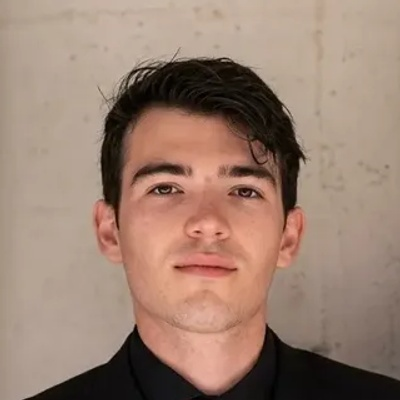
\includegraphics[width=2.3cm,height=2.3cm]{assets/diego-formal.jpg}};
    \end{scope}
    \draw[rulecolor, line width=1.3pt] (0,0) circle (1.15cm);
  \end{tikzpicture}
\end{minipage}

\vspace{1pt}

\section*{Professional Summary}
{\small Bioinformatics graduate and Master's student in Computer Engineering. Passionate about technology and developing independent projects. Specialized in software engineering, data architectures, and infrastructure. Seeking a collaborative environment that fosters continuous learning where I can contribute technical value to innovative initiatives.}

\section*{Professional Experience}

\noindent\textbf{Software Engineer, Khaos Research} \hfill {\footnotesize\color{subtext}\textbf{Sept 2025 -- Present}} \\
{\footnotesize\color{subtext}\textit{R\&D on European federated data spaces (SEDIA \textbar\ Gaia-X)}}
\begin{itemize}
  \item Designed and integrated a hybrid search engine combining vector retrieval in \textbf{Qdrant} and lexical search, supported by knowledge-graph agents to navigate data spaces.
  \item Proposed and developed a metadata extraction and cataloging tool, evolving into an independent project with an ongoing scientific publication.
  \item Optimized data ingestion pipelines for large-scale datasets used to train a predictive model on Sentinel-2 satellite imagery.
\end{itemize}

\vspace{5pt}

\noindent\textbf{Full-Stack Developer, mSurgery} \hfill {\footnotesize\color{subtext}\textbf{March 2025 -- July 2025}} \\
{\footnotesize\color{subtext}\textit{Medical telemetry platforms and real-time surgical digital twins}}
\begin{itemize}
  \item Led the frontend migration to \textbf{Svelte 5}, adopting the reactive runes paradigm.
  \item Delivered technical demonstrations and presentations in English to international investors and industry committees at the National Digital Content Hub.
\end{itemize}

\vspace{5pt}

\noindent\textbf{Junior Software Engineer, T\&B Company Group} \hfill {\footnotesize\color{subtext}\textbf{June 2021 -- December 2021}} \\
{\footnotesize\color{subtext}\textit{Corporate platform modernization toward REST microservices}}
\begin{itemize}
  \item Refactored legacy modules in Java and Angular toward decoupled architectures.
  \item Designed standard interface contracts with \textbf{OpenAPI / Swagger} and documented REST microservices to accelerate frontend-backend team integration.
\end{itemize}

\section*{Selected Technical Projects \hfill {\normalfont\scriptsize\color{subtext}\href{https://diegodepablo.is-a.dev/projects}{\csname faExternalLink*\endcsname\ diegodepablo.is-a.dev/projects}}}

\noindent\textbf{\href{https://diegodepablo.is-a.dev/projects/tfg-patient-monitoring}{\csname faExternalLink*\endcsname\ Biomedical Telemonitoring IoT Wristband (B.Sc. Thesis)}} \hfill {\scriptsize\color{subtext}\textbf{Stack:} C++, FreeRTOS, ESP32, MQTT, FastAPI, TimescaleDB, Docker}
\begin{itemize}
  \item End-to-end telemonitoring prototype: multithreaded ESP32 firmware for vital signs via photoplethysmography (pulse and SpO2) and fall detection algorithm using MPU-6050 accelerometer.
  \item Wireless synchronization pipeline over MQTT to a FastAPI backend and TimescaleDB with a real-time web dashboard. \textbf{Grade:} 10/10 with Honors.
\end{itemize}

\vspace{4.5pt}

\noindent\textbf{\href{https://diegodepablo.is-a.dev/projects/titan-workflow}{\csname faExternalLink*\endcsname\ TITAN Workflow: Scientific Workflow Orchestrator \& Assistant}} \hfill {\scriptsize\color{subtext}\textbf{Stack:} FastAPI, Pydantic AI, LangChain, LLMs, Docker}
\begin{itemize}
  \item Intelligent assistant for scientific workflow composition and validation: verifies data schemas and dependency compatibility prior to execution using Pydantic AI validators.
\end{itemize}

\section*{Education}

\noindent\textbf{M.Sc. in Computer Engineering} \textbar\ \textit{University of Malaga} \hfill {\footnotesize\color{subtext}\textbf{2026 -- Present}} \\[2.5pt]
\noindent\textbf{B.Sc. in Health Engineering (Bioinformatics Specialization)} \textbar\ \textit{University of Malaga} \hfill {\footnotesize\color{subtext}\textbf{Sep 2021 -- Jul 2025}} \\
{\footnotesize GPA: \textbf{7.96/10}. Honors in \textit{Programming Fundamentals}, \textit{Intelligent Systems}, and \textit{Bioinformatics Projects}. Thesis graded \textbf{10/10 with Honors}.}

\section*{Technical Skills \& Languages}

{\footnotesize
\noindent\textbf{Programming Languages:} Python, JavaScript, TypeScript, C\#, SQL, Java, Bash, R. \\[2.5pt]
\textbf{Backend \& Architecture:} FastAPI, REST Microservices, OpenAPI / Swagger, Pydantic, Concurrency (AsyncIO), Node.js. \\[2.5pt]
\textbf{Databases \& Search:} PostgreSQL, Elasticsearch, Qdrant (Vector DB), Redis. \\[2.5pt]
\textbf{AI, DevOps \& Systems:} Pydantic AI, LangChain, RAG / Embeddings, LLM Agents, PyTorch, Docker, Kubernetes, Helm, Argo CD, CI/CD, Linux. \\[2.5pt]
\textbf{Frontend \& UI:} React, Svelte 5, Next.js, HTML5, CSS, Tailwind CSS. \hfill \textbf{Languages:} \textbf{Spanish} (Native) \enskip $\cdot$ \enskip \textbf{English} (B2 Professional).
}

\end{document}
